\documentclass[11pt]{article}
%DIF LATEXDIFF DIFFERENCE FILE
%DIF DEL bayesianflows_arxiv_fordiff.tex   Mon Aug  5 18:18:51 2024
%DIF ADD bayesianflows.tex                 Tue Apr 15 18:28:30 2025
\usepackage[top=1.00in, bottom=1.0in, left=1in, right=1in]{geometry}
%DIF 3c3
%DIF < \renewcommand{\baselinestretch}{1.1}
%DIF -------
\renewcommand{\baselinestretch}{1.9} %DIF > 
%DIF -------
\usepackage{graphicx}
\usepackage{natbib}
\usepackage{amsmath}
%DIF 7a7-8
\usepackage{gensymb} %DIF > 
\usepackage{xcolor} %DIF > 
%DIF -------
\usepackage{xr-hyper}
%DIF 8a10
\externaldocument{bayesianflowsysupp} %DIF > 
%DIF -------
\usepackage{hyperref}
%DIF 9a12
\usepackage{lineno} %DIF > 
%DIF -------

\def\labelitemi{--}

\usepackage{fancyhdr}
\pagestyle{fancy}
\fancyhead[LO]{}
\fancyhead[RO]{}
%DIF PREAMBLE EXTENSION ADDED BY LATEXDIFF
%DIF UNDERLINE PREAMBLE %DIF PREAMBLE
\RequirePackage[normalem]{ulem} %DIF PREAMBLE
\RequirePackage{color}\definecolor{RED}{rgb}{1,0,0}\definecolor{BLUE}{rgb}{0,0,1} %DIF PREAMBLE
\providecommand{\DIFaddtex}[1]{{\protect\color{blue}\uwave{#1}}} %DIF PREAMBLE
\providecommand{\DIFdeltex}[1]{{\protect\color{red}\sout{#1}}}                      %DIF PREAMBLE
%DIF SAFE PREAMBLE %DIF PREAMBLE
\providecommand{\DIFaddbegin}{} %DIF PREAMBLE
\providecommand{\DIFaddend}{} %DIF PREAMBLE
\providecommand{\DIFdelbegin}{} %DIF PREAMBLE
\providecommand{\DIFdelend}{} %DIF PREAMBLE
\providecommand{\DIFmodbegin}{} %DIF PREAMBLE
\providecommand{\DIFmodend}{} %DIF PREAMBLE
%DIF FLOATSAFE PREAMBLE %DIF PREAMBLE
\providecommand{\DIFaddFL}[1]{\DIFadd{#1}} %DIF PREAMBLE
\providecommand{\DIFdelFL}[1]{\DIFdel{#1}} %DIF PREAMBLE
\providecommand{\DIFaddbeginFL}{} %DIF PREAMBLE
\providecommand{\DIFaddendFL}{} %DIF PREAMBLE
\providecommand{\DIFdelbeginFL}{} %DIF PREAMBLE
\providecommand{\DIFdelendFL}{} %DIF PREAMBLE
%DIF HYPERREF PREAMBLE %DIF PREAMBLE
\providecommand{\DIFadd}[1]{\texorpdfstring{\DIFaddtex{#1}}{#1}} %DIF PREAMBLE
\providecommand{\DIFdel}[1]{\texorpdfstring{\DIFdeltex{#1}}{}} %DIF PREAMBLE
\newcommand{\DIFscaledelfig}{0.5}
%DIF HIGHLIGHTGRAPHICS PREAMBLE %DIF PREAMBLE
\RequirePackage{settobox} %DIF PREAMBLE
\RequirePackage{letltxmacro} %DIF PREAMBLE
\newsavebox{\DIFdelgraphicsbox} %DIF PREAMBLE
\newlength{\DIFdelgraphicswidth} %DIF PREAMBLE
\newlength{\DIFdelgraphicsheight} %DIF PREAMBLE
% store original definition of \includegraphics %DIF PREAMBLE
\LetLtxMacro{\DIFOincludegraphics}{\includegraphics} %DIF PREAMBLE
\newcommand{\DIFaddincludegraphics}[2][]{{\color{blue}\fbox{\DIFOincludegraphics[#1]{#2}}}} %DIF PREAMBLE
\newcommand{\DIFdelincludegraphics}[2][]{% %DIF PREAMBLE
\sbox{\DIFdelgraphicsbox}{\DIFOincludegraphics[#1]{#2}}% %DIF PREAMBLE
\settoboxwidth{\DIFdelgraphicswidth}{\DIFdelgraphicsbox} %DIF PREAMBLE
\settoboxtotalheight{\DIFdelgraphicsheight}{\DIFdelgraphicsbox} %DIF PREAMBLE
\scalebox{\DIFscaledelfig}{% %DIF PREAMBLE
\parbox[b]{\DIFdelgraphicswidth}{\usebox{\DIFdelgraphicsbox}\\[-\baselineskip] \rule{\DIFdelgraphicswidth}{0em}}\llap{\resizebox{\DIFdelgraphicswidth}{\DIFdelgraphicsheight}{% %DIF PREAMBLE
\setlength{\unitlength}{\DIFdelgraphicswidth}% %DIF PREAMBLE
\begin{picture}(1,1)% %DIF PREAMBLE
\thicklines\linethickness{2pt} %DIF PREAMBLE
{\color[rgb]{1,0,0}\put(0,0){\framebox(1,1){}}}% %DIF PREAMBLE
{\color[rgb]{1,0,0}\put(0,0){\line( 1,1){1}}}% %DIF PREAMBLE
{\color[rgb]{1,0,0}\put(0,1){\line(1,-1){1}}}% %DIF PREAMBLE
\end{picture}% %DIF PREAMBLE
}\hspace*{3pt}}} %DIF PREAMBLE
} %DIF PREAMBLE
\LetLtxMacro{\DIFOaddbegin}{\DIFaddbegin} %DIF PREAMBLE
\LetLtxMacro{\DIFOaddend}{\DIFaddend} %DIF PREAMBLE
\LetLtxMacro{\DIFOdelbegin}{\DIFdelbegin} %DIF PREAMBLE
\LetLtxMacro{\DIFOdelend}{\DIFdelend} %DIF PREAMBLE
\DeclareRobustCommand{\DIFaddbegin}{\DIFOaddbegin \let\includegraphics\DIFaddincludegraphics} %DIF PREAMBLE
\DeclareRobustCommand{\DIFaddend}{\DIFOaddend \let\includegraphics\DIFOincludegraphics} %DIF PREAMBLE
\DeclareRobustCommand{\DIFdelbegin}{\DIFOdelbegin \let\includegraphics\DIFdelincludegraphics} %DIF PREAMBLE
\DeclareRobustCommand{\DIFdelend}{\DIFOaddend \let\includegraphics\DIFOincludegraphics} %DIF PREAMBLE
\LetLtxMacro{\DIFOaddbeginFL}{\DIFaddbeginFL} %DIF PREAMBLE
\LetLtxMacro{\DIFOaddendFL}{\DIFaddendFL} %DIF PREAMBLE
\LetLtxMacro{\DIFOdelbeginFL}{\DIFdelbeginFL} %DIF PREAMBLE
\LetLtxMacro{\DIFOdelendFL}{\DIFdelendFL} %DIF PREAMBLE
\DeclareRobustCommand{\DIFaddbeginFL}{\DIFOaddbeginFL \let\includegraphics\DIFaddincludegraphics} %DIF PREAMBLE
\DeclareRobustCommand{\DIFaddendFL}{\DIFOaddendFL \let\includegraphics\DIFOincludegraphics} %DIF PREAMBLE
\DeclareRobustCommand{\DIFdelbeginFL}{\DIFOdelbeginFL \let\includegraphics\DIFdelincludegraphics} %DIF PREAMBLE
\DeclareRobustCommand{\DIFdelendFL}{\DIFOaddendFL \let\includegraphics\DIFOincludegraphics} %DIF PREAMBLE
%DIF COLORLISTINGS PREAMBLE %DIF PREAMBLE
\RequirePackage{listings} %DIF PREAMBLE
\RequirePackage{color} %DIF PREAMBLE
\lstdefinelanguage{DIFcode}{ %DIF PREAMBLE
%DIF DIFCODE_UNDERLINE %DIF PREAMBLE
  moredelim=[il][\color{red}\sout]{\%DIF\ <\ }, %DIF PREAMBLE
  moredelim=[il][\color{blue}\uwave]{\%DIF\ >\ } %DIF PREAMBLE
} %DIF PREAMBLE
\lstdefinestyle{DIFverbatimstyle}{ %DIF PREAMBLE
	language=DIFcode, %DIF PREAMBLE
	basicstyle=\ttfamily, %DIF PREAMBLE
	columns=fullflexible, %DIF PREAMBLE
	keepspaces=true %DIF PREAMBLE
} %DIF PREAMBLE
\lstnewenvironment{DIFverbatim}{\lstset{style=DIFverbatimstyle}}{} %DIF PREAMBLE
\lstnewenvironment{DIFverbatim*}{\lstset{style=DIFverbatimstyle,showspaces=true}}{} %DIF PREAMBLE
%DIF END PREAMBLE EXTENSION ADDED BY LATEXDIFF

\begin{document}
\DIFaddbegin \bibliographystyle{/Users/Lizzie/Documents/EndnoteRelated/Bibtex/styles/amnat}
\renewcommand{\refname}{\CHead{}}
\DIFaddend 

%DIF > %%%%%%
%DIF > % To do %%
%DIF > %%%%%%
%DIF >  https://github.com/lizzieinvancouver/gelmanhill/wiki/Vocabulary
\DIFaddbegin 

{\Large \DIFadd{A four-step Bayesian workflow for improving ecological science}}\\
\vspace{3ex}

\iffalse %DIF >  remember to also add back in the acknowledgements 
\DIFaddend \title{A four-step Bayesian workflow for improving ecological science}
%DIF >  Simulation as a best practice in Bayesian workflows and beyond
%DIF >  How to fit Bayesian models and influence people
%DIF >  How to do Bayesian model fitting in ecology 
%DIF >  The best way to be a Bayesian in ecology today
%DIF >  \date{\today}
\author{EM Wolkovich$^{1*}$, T Jonathan Davies$^{1,2}$, William D Pearse$^{3,4}$ \& Michael Betancourt$^{5}$}
\maketitle

\noindent $^{1}$ Forest and Conservation Sciences, University of British Columbia, Vancouver, BC V6T 1Z4, Canada\\
$^{2}$ Botany, University of British Columbia, Vancouver, BC V6T 1Z4, Canada\\
$^{3}$ Department of Life Sciences, Imperial College London, Ascot SL5 7PY, United Kingdom \\
$^{4}$ Alan Turing Institute, British Library, 96 Euston Road, London NW1 2DB, United Kingdom \\
$^{5}$ Symplectomorphic, LLC, New York, NY 10026, USA \\
$^{*}$ \url{mailto: e.wolkovich@ubc.ca}
\DIFdelbegin %DIFDELCMD < 

%DIFDELCMD < %%%
\DIFdelend \DIFaddbegin \fi 
\DIFaddend \vspace{3ex}
\noindent \emph{Keywords:} big data; scientific workflow; data simulation; forecasting; null hypothesis testing
\vspace{3ex}

%DIF >  \noindent \emph{Data availability:} No new data, but full code and raw data are provided in the supplement for an example workflow.
\noindent\emph{\DIFaddbegin \DIFadd{Example \& }\DIFaddend Data\DIFdelbegin \DIFdel{availability}\DIFdelend :} \DIFdelbegin \DIFdel{No new data, but full code and raw data are provided in the supplement for an example workflow. }\DIFdelend \DIFaddbegin \DIFadd{We provide an example of the workflow with complete code available eventually on its GitHub site, but for double-blind review we provide it here as a compressed set of files.  The data used for the example is provided and full metadata on it is available via the Knowledge Network for Biocomplexity: }{\color{blue}%DIFAUXCMD
\verb|doi:10.5063/F12J69B2|%
}%DIFAUXCMD
\DIFadd{. %DIF >  \url{https://github.com/lizzieinvancouver/bayesianflowsexample};
}\DIFaddend 

\newpage
\DIFaddbegin \linenumbers
%DIF >  about 140 words (200 max for NEE); main text is 4,000; 3-4K for a perspective, see https://www.nature.com/natecolevol/content
%DIF >  Or submit to ELE as method: https://onlinelibrary.wiley.com/page/journal/14610248/homepage/forauthors.html#tips2
%DIF >  Mid Jan 2024  >7,000 words // 4 Feb 2024: Down to 5023 // 7 April 2024: 4859 // 27 May 2024: 3713 // 26 Sept 2024: 2685
\abstract{Growing anthropogenic pressures have increased the need for robust predictive models. Meeting this demand requires approaches that can handle bigger data to yield forecasts that capture the variability and underlying uncertainty of ecological systems. Bayesian models are especially adept at this and are growing in use in ecology. Yet many ecologists are not trained in current methods to build flexible robust models. 
% Yet many ecologists today are not trained to take advantage of the bigger ecological data needed to generate more flexible robust models. 
Here we describe a broadly generalizable workflow for statistical analyses and show how it can enhance training in ecology. 
% Here we describe a broadly generalizable workflow for statistical analyses centered on simulating data from models, and show how it can enhance training in ecology. 
Building on the increasingly computational toolkit of many ecologists, this approach leverages simulation to integrate model building and testing for empirical data more fully with ecological theory.  In turn this workflow can fit models that are more robust and well-suited to provide new ecological insights---allowing us to refine where to put resources for better estimates, better models, and better forecasts.}
%DIF >  OLD version of second half (including our Bayesian beach): Here we present a Bayesian workflow---centered on simulating data from models---that represents a ground shift of not just how to fit Bayesian models, but how we should approach model fitting to advance our science. This workflow integrates mechanistic and statistical models with a computational toolkit, which we argue can accelerate ecological science. By interrogating our methods through generative models, we can refine where to put resources for better estimates, better models, and better forecasts. While we outline these methods from the happy surf of our Bayesian beach, the ocean we describe works for anyone fitting models to ecological data.
\DIFaddend 



\DIFdelbegin %DIFDELCMD < \abstract{Growing anthropogenic pressures have increased the need for robust predictive models. Meeting this demand requires approaches that can handle bigger data to yield forecasts that capture the variability and underlying uncertainty of ecological systems. Bayesian models are especially adept at this and are growing in use in ecology. Yet many ecologists today are not trained to take advantage of the bigger ecological data needed to generate more flexible robust models. Here we describe a broadly generalizable workflow for statistical analyses and show how it can enhance training in ecology. Building on the increasingly computational toolkit of many ecologists, this approach leverages simulation to integrate model building and testing for empirical data more fully with ecological theory.  In turn this workflow can fit models that are more robust and well-suited to provide new ecological insights---allowing us to refine where to put resources for better estimates, better models, and better forecasts.}
%DIFDELCMD < 

%DIFDELCMD < %%%
\DIFdelend \setlength{\parindent}{0pt}
\setlength{\parskip}{7pt}

\DIFaddbegin \newpage

\DIFaddend \section*{Introduction}
In recent years, as ecologists have worked to develop global predictive models, they have developed ever larger datasets \citep{Hampton2013}. These bigger data, however, are also messier data. Such data generally requires a model of both the underlying biological processes and how the measurements were made. Some fields have long used these types of models \DIFdelbegin \DIFdel{\mbox{%DIFAUXCMD
\citep[generally in fields focused on inferring population sizes of things people want to eat or manage,][]{muthuku2008,zheng2007,trijoulet2018,strinella2020potential}}\hskip0pt%DIFAUXCMD
}\DIFdelend \DIFaddbegin \DIFadd{\mbox{%DIFAUXCMD
\citep[generally in fields focused on inferring population sizes for management,][]{muthuku2008,zheng2007,trijoulet2018,strinella2020potential}}\hskip0pt%DIFAUXCMD
}\DIFaddend . Most, however, have not. This has left many researchers to try to adapt what they were trained in---traditional statistical methods (e.g. $F$ and $t$ tests) and a strong focus on null hypothesis testing---to increasingly complex datasets. 
\DIFdelbegin \DIFdel{Often they have done this by fitting multi-way interaction terms, using random effects to correct for group level factors, or comparing across a large suite of models. 
}\DIFdelend %DIF >  Often they have done this by fitting multi-way interaction terms, using random effects to correct for group level factors, or comparing across a large suite of models. 
%DIF >  Often they have done this by fitting multi-way interaction terms (rather than using mechanistic models informed by biological understanding), using random effects to correct for group level factors (rather than explicit models of data-collection biases), or comparing across a large suite of models (because they cannot fit a single model that accounts for all the idiosyncrasies and biases) ... and so aim to average out the noise to leave only the signal 

\DIFdelbegin \DIFdel{Common embedded }\DIFdelend \DIFaddbegin \DIFadd{Yet many common }\DIFaddend statistical approaches do not \DIFdelbegin \DIFdel{often }\DIFdelend align with ecology's aims today. Beyond the reality that most traditional methods are fragile when used beyond the cleaner, simpler experiments these methods assume (e.g. spatial, temporal and phylogenetic correlations often violate \DIFdelbegin \DIFdel{common }\DIFdelend independence assumptions), they will usually fail to produce robust, reproducible results. \DIFdelbegin \DIFdel{Multi-way interaction terms can make main effects hard to interpret and require much larger sample sizes to estimate reliably. Null hypotheses are rarely true and can lead to confusion over what is scientifically important versus `significant' \mbox{%DIFAUXCMD
\citep{gelmanhill,muff2022rewriting}}\hskip0pt%DIFAUXCMD
. Many model comparison and machine learning approaches prefer modelswhose inferences match the idiosyncrasies and biases in the available data, but don’t generalize }\DIFdelend \DIFaddbegin \DIFadd{For example, an overly zealous focus on $p$-values has led to a replication crises in several fields, where results seem most likely the outcome of noisy data combined with a search for statistical significance through many models \mbox{%DIFAUXCMD
\citep[effectively a garden of forking paths,][]{halsey2015,loken2017}}\hskip0pt%DIFAUXCMD
. Some model selection approaches, including new machine learning methods, try to avoid this by comparing across models, but may not generalize to provide useful forecasts.  This is especially true when forecasts have to adapt to changes in the underlying biology}\DIFaddend .
\DIFdelbegin \DIFdel{The disconnect between the traditional statistical tools available in ecology and the field's fundamental theory is being made ever-clearer as the need for robust ecological forecasts grows. 
}\DIFdelend 

Bayesian approaches provide a pathway to build powerful models that can transform how we understand our systems as largescale ecological data become increasingly available. Recognizing this, many in ecology are increasingly using Bayesian methods \citep{anderson2021trends}. New algorithms \citep[e.g. Hamiltonian Monte Carlo,][]{nuts2014,betan2019} that have made fitting and implementing Bayesian models faster, more robust and---in many ways---easier \citep{Carpenter:2017stan}. Fitting larger and sometimes more complex models, however, presents challenges that are frequently not addressed in traditional ecological training. We suggest that many of these challenges can be overcome by approaching analyses through specific workflows \citep{betanworkflow,grinsztajn2021,vandeschoot2021}, which themselves are built on a process of how to do not just statistics, but how to do science \citep{box1976science}. 

Such approaches move away from a focus on null hypothesis testing, towards estimating effect sizes, using models calibrated (see Table \ref{tab:glossary}) and better understood through simulating data at multiple \DIFdelbegin \DIFdel{steps---using a number of skills often reserved in ecology more for `theorists' than empirical ecologists. But this theoretical-vs-empirical divide ignores that the average modern ecologist is computational, and thus already has many of the basic skills to build bespoke models. 
}%DIFDELCMD < 

%DIFDELCMD < %%%
\DIFdel{Here we provide }\DIFdelend \DIFaddbegin \DIFadd{steps. %DIF > ---using a number of skills often reserved in ecology more for `theorists' than empirical ecologists.  But this theoretical-vs-empirical divide ignores that the average modern ecologist is computational, and thus already has many of the basic skills to build bespoke models. 
Here we outline }\DIFaddend a simplified---but powerful---workflow that builds on new insights from statistics  \citep{betanworkflow,vandeschoot2021} and the increasingly computational nature of ecology today. \DIFdelbegin \DIFdel{By integrating bespoke model building more fully with ecological theory and understanding---and vice versa---this approach can fit models that are more robust and better-suited to providing new ecological insights and improved predictions}\DIFdelend \DIFaddbegin \DIFadd{Our aim is to provide an approachable rubric for those new to fitting complex models, and is not intended to be a comprehensive overview (see `Next steps' in the Supplement)}\DIFaddend . We introduce our workflow assuming a Bayesian statistical framework \DIFaddbegin \DIFadd{(with an example in the supplement shown in }\textsf{\DIFadd{R}} \DIFadd{and }\textsf{\DIFadd{Stan}}\DIFadd{)}\DIFaddend ; however, it can \DIFdelbegin \DIFdel{also }\DIFdelend be applied to other statistical inference methods. 
%DIF >  Our aim is not to provide a comprehensive overview, but instead to provide an approachable rubric for those new to fitting complex models. 
%DIF >  By integrating bespoke model building more fully with ecological theory and understanding---and vice versa---this approach can fit models that are more robust and better-suited to providing new ecological insights and improved predictions.% After outlining the workflow, we discuss how it has improved our own science, and suggests a new way to train in ecology.
%DIF >  Once you start doing this workflow, your scientific life will never be the same. 

\section*{A basic Bayesian workflow}
\DIFdelbegin \DIFdel{Statistical analyses are designed for inference---to learn about some process, effect or behavior from data. Robust analyses yield inferences consistent with the underlying truth more often than not (quantifying this consistency is called calibration, and is a critical part of using models for inference, see Table \ref{tab:glossary}). Because we do not know the `truth' how we approach our analyses---and our inference---is a critical component of how we do science. Fragile statistical analyses can lead science away from the type of repeatable and generalizable findings expected when inferences align with the truth. For example, an overly zealous focus on $p$-values has led to a replication crises in several fields, where results seem most likely the outcome of noisy data combined with a search for statistical significance through many models \mbox{%DIFAUXCMD
\citep[effectively a garden of forking paths,][]{halsey2015,loken2017}}\hskip0pt%DIFAUXCMD
. Some model selection approaches, including new machine learning methods, try to avoid this by comparing across models, but may not generalize to provide useful forecasts.  This is especially true when forecasts have to adapt to changes in the underlying ecology.
}\DIFdelend %DIF >  \section*{A short guide to statistical workflows and Bayesian approaches}
%DIF >  Statistical analyses are designed for inference---to learn about some process, effect or behavior from data. Robust analyses yield inferences consistent with the underlying truth more often than not (quantifying this consistency is called calibration, and is a critical part of using models for inference, see Table \ref{tab:glossary}). Because we do not know the `truth' how we approach our analyses---and our inference---is a critical component of how we do science. Fragile statistical analyses can lead science away from the type of repeatable and generalizable findings expected when inferences align with the truth. 

\DIFdelbegin \DIFdel{We argue that robust analyses comes from explicitly building and challenging a model (or set of models ) in an organized sequence of steps---a workflow. We outline one such workflow using a Bayesian approach (with an example in the supplement shown in }\textsf{\DIFdel{R}} %DIFAUXCMD
\DIFdel{and }\textsf{\DIFdel{Stan}}%DIFAUXCMD
\DIFdel{). }%DIFDELCMD < 

%DIFDELCMD < %%%
\DIFdel{In ecology, Bayesian methods often shift focus away from null hypothesis testing and point estimates and towards evaluating more fully a model's output, including uncertainty---often using a specific model designed for the system and question at hand. These bespoke }\DIFdelend \DIFaddbegin \DIFadd{Our workflow outlines what we consider the major steps for building bespoke models (Fig. \ref{fig:workflow}). Such }\DIFaddend models can be fit by applying Bayes' theorem, which generates a $posterior$ distribution from a combination of a $likelihood$ and a $prior$ distribution (an initial uncertainty estimate derived from basic ecological knowledge), and using iterative algorithms (e.g. MCMC, Markov Chain Monte Carlo) that provide samples that can be used to extract information from the posterior distribution (for more, see \emph{A brief review of statistical inference using Bayesian approaches} in the Supplement). \DIFdelbegin %DIFDELCMD < 

%DIFDELCMD < %%%
\DIFdel{Our workflow describes what we consider the major steps for Bayesian model fitting (Fig. \ref{fig:workflow}). This includes model development (Step 1) and calibration (Step 2), inference (Step 3), and then model improvement (Step 4). }\DIFdelend Many of these steps will be familiar to statistical ecologists, but are often overlooked, whereas other steps may appear particular to Bayesian methods (e.g. prior predictive checks), but are actually useful for anyone---using Bayesian models or not---to challenge their models of how the world works. Parts of this workflow could be \DIFdelbegin \DIFdel{dropped, or }\DIFdelend expanded as workflows in themselves, given other aims (see Supplement: Which workflow?). \DIFdelbegin \DIFdel{For simplicity. many of the smaller but still critical steps are omitted, including visualization, which is required at every step \mbox{%DIFAUXCMD
\citep[and for which there are many good resources, e.g.][]{gabryvis}}\hskip0pt%DIFAUXCMD
. 
}\DIFdelend %DIF >  For simplicity, many of the smaller but still critical steps are omitted, including visualization, which is required at every step \citep[and for which there are many good resources, e.g.][]{gabryvis}. 

\subsection*{Step 1: Develop your model(s)} 

We start the workflow with what can feel like the biggest step---build a model (or potentially, models) \DIFdelbegin \DIFdel{that you want to fit your data to }\DIFdelend based on your aims. By developing a model designed for your biological question, data and aims, your statistical workflow naturally becomes a scientific workflow. You will more clearly see the assumptions and mechanisms in your model, which is especially valuable given how often our intuition of how models `work' is wrong \citep{kokko2005useful}. \DIFdelbegin %DIFDELCMD < 

%DIFDELCMD < %%%
\DIFdelend You likely already have a model, though it may be only verbal or conceptual. For this workflow, however, you’ll need to convert such models into mathematical versions \citep{servedio2014not}. \DIFdelbegin \DIFdel{This step is better }\DIFdelend %DIF >  This step is better approached before you collect your data. After data collection, it becomes far more tempting to focus on the particular details in the data and not the latent processes and biological models from which the data were generated. 
\DIFaddbegin 

\DIFadd{Though it can feel challenging at first, this step is best }\DIFaddend approached before you collect \DIFdelbegin \DIFdel{your data. After data collection, it becomes far more tempting to focus on the particular details in the data and not the latent processes and biological models from which the data were generated. 
}%DIFDELCMD < 

%DIFDELCMD < %%%
\DIFdel{Getting to the point where this step is part of your data design and collection, however, requires starting somewhere---with some model (or models) in hand. }\DIFdelend \DIFaddbegin \DIFadd{any data. }\DIFaddend A suite of resources for `generative' or `narratively generative' modeling can help \citep{statrethink,betangen}\DIFdelbegin \DIFdel{, along with two points. First, know that you can and will improve on this skill. Second, as you }\DIFdelend \DIFaddbegin \DIFadd{. %DIF >  along with two points. First, know that you can and will improve on this skill. 
As you }\DIFaddend start, ask lots of questions---and push yourself on your answers---about what you expect and what's reasonable biologically from your model. \DIFdelbegin \DIFdel{For example, instead of simply identifying which distribution your observed response variable looks most similar to, ask yourself what ecological processes generate that distribution and how they influence its properties (e.g. its mean, minimum and maximum). Do you expect data below zero? Up to infinity? If not, why not? Effective model building is about efficient brainstorming and this is a critical part of the process. 
}%DIFDELCMD < 

%DIFDELCMD < %%%
\DIFdelend %DIF >  For example, instead of simply identifying which distribution your observed response variable looks most similar to, ask yourself what ecological processes generate that distribution and how they influence its properties (e.g. its mean, minimum and maximum). Do you expect data below zero? Up to infinity? If not, why not? Effective model building is about efficient brainstorming and this is a critical part of the process. 
As you do this, you'll be generating your model---including its priors, which are important for Bayesian analysis. Assigning priors generally forces you to think about your model with regards to your study system, and interrogate what's probable, possible or actually \DIFdelbegin \DIFdel{unreasonable. While many packages (e.g. }\textsf{\DIFdel{brms, rstanarm}}%DIFAUXCMD
\DIFdel{, which fit a suite of pre-defined models) will automatically set default priors, assigning them yourself }\DIFdelend \DIFaddbegin \DIFadd{unreasonable---and }\DIFaddend can quickly disabuse users of \DIFdelbegin \DIFdel{their prejudices }\DIFdelend \DIFaddbegin \DIFadd{prejudices regarding priors}\DIFaddend . For example, you may not think you have a prior on how sunlight affects plant growth, until you realize your `agnostic prior' actually allows plants to grow hundreds of meters per day. %DIF >  You can take this a step up with Step 2's prior predictive checks. % something like `and generally this will not impact your results, see Supp'

\subsection*{Step 2: Check your model on simulated data} 

Once you have your model and its priors jotted down, you need to write up your model in a particular modeling language and check it. As with all code: just because it runs, does not mean it does what you think it does. The worst errors often still permit code to run. \DIFdelbegin \DIFdel{Whether writing it out in }\textsf{\DIFdel{Stan}}%DIFAUXCMD
\DIFdel{, where you need to be able to write out the full likelihood and set all your own priors, or using a package that writes much of the model for you (e.g. }\textsf{\DIFdel{rstanarm}}%DIFAUXCMD
\DIFdel{), you need a way to verify the code is correct: test data.
}\DIFdelend %DIF >  Whether writing it out in \textsf{Stan}, where you need to be able to write out the full likelihood and set all your own priors, or using a package that writes much of the model for you (e.g. \textsf{rstanarm}), you need a way to verify the code is correct: test data.

Test data (aka `simulated data', or  `fake data,' etc.), and the skills required to build it, are central to this workflow. With `test data' you simulate data from your model in such a way that you can use the resulting data to test if your model code is correct (i.e., you fix values for your model parameters, then test how well your model recovers them, see the Supplement for an example). While there's no guarantee that inferences will always recover the parameter values you set, even when using the correct model, extreme disagreement is often an indicator that something is amiss in the implementation of the model. At the same time these simulation studies can help understand how often a model might lead to the correct inference (see Fig. \ref{fig:misspecifyprior}). As you do this, you will also be calibrating your model---seeing how accurately and precisely it estimates parameters \DIFdelbegin \DIFdel{you set }\DIFdelend and under what conditions. 

This very basic model checking step is uncommon for many ecologists, but critical in our view. If you can simulate data from your model, then you can powerfully---and easily---answer questions related to statistical power, what effect sizes are reasonable, and---most likely---have new insights into how your model suggests the world works, all before looking at any real data. \DIFdelbegin \DIFdel{`All models are wrong; some models are useful, ' becomes much clearer when you have the power to generate data from your model under any parameter set and sample size you want. Conversely, if you cannot complete this step, you'll struggle to understand if the model fits well, and struggle further to meaningfully interpret the model output, making an }\DIFdelend \DIFaddbegin \DIFadd{Thus, this }\DIFaddend apparently simple programmatic task actually \DIFdelbegin \DIFdel{encapsulate }\DIFdelend \DIFaddbegin \DIFadd{encapsulates }\DIFaddend a far deeper understanding of your model. %DIF >  `All models are wrong; some models are useful,' becomes much clearer when you have the power to generate data from your model under any parameter set and sample size you want. 

You can learn only so much, however, from data simulated from a particular parameter set. Simulation studies across multiple parameter sets allow you to investigate how robust your inferential performance might be. Prior predictive checks \DIFaddbegin \DIFadd{\mbox{%DIFAUXCMD
\citep{betanprior,wesner2021,winter2023} }\hskip0pt%DIFAUXCMD
}\DIFaddend use the Bayesian prior model to set this scope of such simulations. For these, you draw values from your prior distribution \DIFdelbegin \DIFdel{(usually randomly in your code) }\DIFdelend and then explore how your model performs\DIFdelbegin \DIFdel{under those draws}\DIFdelend . Seeing how this influences your resulting output reveals the extent to which your model can capture known variation in your data, and gives insight into whether your model is capable of distinguishing among competing hypotheses. \DIFdelbegin \DIFdel{It also serves as a check on the priors you're using (addressing one of the common concerns of those inexperienced with Bayesian models). How exactly to do this depends on your question, model and aims, but many guides can help you think through this \mbox{%DIFAUXCMD
\citep{betanprior,wesner2021,winter2023}}\hskip0pt%DIFAUXCMD
. }%DIFDELCMD < \\
%DIFDELCMD < %%%
\DIFdelend %DIF >  It also serves as a check on the priors you're using (addressing one of the common concerns of those inexperienced with Bayesian models). 


 \subsection*{Step 3: Run your model on your empirical data} 

The next step is to run the model---you've now \DIFdelbegin \DIFdel{validated}\DIFdelend \DIFaddbegin \DIFadd{evaluated}\DIFaddend , test-run and have ready to go---on your exciting new empirical data. Check diagnostics so you know it's running well and adjust until it is \citep[this includes a suite of convergence and efficiency metrics that are well-discussed elsewhere,][]{betanworkflow,gelman2020bayesian,vandeschoot2021,gabryvis}. \DIFdelbegin \DIFdel{A model that doesn't converge, or seems to suggest coefficients that are completely at odds with the data, can result from a model that was mis-specified and could never capture real-world variation. For serious problems you may need to reevaluate your model entirely and return to Steps 1 and 2.
 }\DIFdelend %DIF >  A model that doesn't converge, or seems to suggest coefficients that are completely at odds with the data, can result from a model that was mis-specified and could never capture real-world variation. For serious problems you may need to reevaluate your model entirely and return to Steps 1 and 2.

This is the step many ecologists skip straight to, ourselves included. It's easy to see the appeal: this is the inference step and where you \DIFdelbegin \DIFdel{have the opportunity to see }\DIFdelend \DIFaddbegin \DIFadd{might gain }\DIFaddend new ecological insights. Fitting new data to the model can feel like the moment when you'll learn something new. But, at least in our experience, this is not always the case. When we rush to this step, that first model we fit is often followed by another, and another---perhaps because one does not converge, or the results of another do not make immediate sense. And with the excitement of getting a model to run we can get distracted from what we are actually most interested in---the inference into ecology. %DIF > In contrast, by approaching the model through Steps 1-2, it's often much easier to quickly see through the results of the model fit. 

Following this workflow can make this step much more satisfying. Here the benefits of the workflow may become excitedly apparent: you have estimates in useful units with uncertainty you can understand. You can use this information to draw new conclusions, design new experiments and more---but this is also a point to stop and check your model. 
%DIF >   As we're all familiar with this step, it's hopefully straightforward. Run the model---you've now validated, test-run and have ready to go---on your exciting new empirical data. Check diagnostics so you know it's running well (convergence metrics, lack of divergent transitions etc.) and tweak until it is. 

\subsection*{Step 4: Check your model on data simulated from your empirical model output (also known as posterior retrodictive checks)} 

%DIF >  Once you have your posterior based on your model and new empirical data, it's time to interrogate it. 
Once you have your posterior based on your model and new empirical data, it's time to remember that it's wrong \DIFdelbegin \DIFdel{, `}\DIFdelend \DIFaddbegin \DIFadd{(as }\DIFaddend all models are\DIFdelbegin \DIFdel{wrong' after all, }\DIFdelend \DIFaddbegin \DIFadd{) }\DIFaddend and ask how useful it is. \DIFdelbegin \DIFdel{You can do some of this through common model-fit diagnostics, such as $R^2$, which compares point predictions to the observed data. With a posterior, however, you can compare an entire distribution of predictions to the observed data. 
}%DIFDELCMD < 

%DIFDELCMD < %%%
\DIFdelend %DIF >  You can do some of this through common model-fit diagnostics, such as $R^2$, which compares point predictions to the observed data. With a posterior, however, you can compare an entire distribution of predictions to the observed data. 
This is where simulating from your model can be especially insightful. It will not only indicate that the model isn't adequately fitting the data but also can suggest what the problems might be. \DIFdelbegin \DIFdel{Steps 1-2 have set you up well for this, as you have a sense of what different parameter estimates do to the model, and test data provide a sense of how it works on data similar to yours. Now with the }\DIFdelend \DIFaddbegin \DIFadd{Using the }\DIFaddend parameter estimates from your posterior \DIFdelbegin \DIFdel{you can }\DIFdelend \DIFaddbegin \DIFadd{to }\DIFaddend simulate new data \DIFdelbegin \DIFdel{from them and }\DIFdelend \DIFaddbegin \DIFadd{\mbox{%DIFAUXCMD
\citep[][]{held2010,gelman200ppc,conn2018} }\hskip0pt%DIFAUXCMD
lets you }\DIFaddend see how that new world compares to the observed data---called posterior retrodictive checks (or posterior predictive checks, Fig. \ref{fig:retrodictivecheck}). 
\DIFdelbegin \DIFdel{Exactly how to do these depend---again---on your question, model and aims \mbox{%DIFAUXCMD
\citep[see][]{held2010,gelman200ppc,conn2018}}\hskip0pt%DIFAUXCMD
. 
}\DIFdelend %DIF >  Steps 1-2 have set you up well for this, as you have a sense of what different parameter estimates do to the model, and test data provide a sense of how it works on data similar to yours. 

Often here you may find big differences from your empirical data, and can start to generate hypotheses for why. For example, you may find patterns that suggest missing grouping factors (e.g. site or biome) through visual posterior retrodictive checks, or you may quickly realize your model predicts impossible numbers for your biological reality. You may begin to see inadequacies in your model, or even potentially your data.  This is one of the main benefits of the workflow: models don't fail silently, they fail with a wealth of context \DIFdelbegin \DIFdel{the }\DIFdelend \DIFaddbegin \DIFadd{that }\DIFaddend helps to generate new models and \DIFdelbegin \DIFdel{better experiments.
}\DIFdelend \DIFaddbegin \DIFadd{experiments.
%DIF >  it helps generate new models and experiments. 
}\DIFaddend 

\subsection*{Feedbacks \& workflows}
A key feature of this workflow is that it can be iterated.  If you find that you want to tweak your model then you \DIFdelbegin \DIFdel{just }\DIFdelend return to the beginning, adjust your model, and repeat the rest of the workflow. In this way, fitting multiple models is encouraged, but this is distinct from the quest for a minimum adequate model or one `best' fit. Feedbacks in this workflow are focused far more on what is biologically reasonable, and understanding the utility---and limits---of inference from your data for your model.  And there are big benefits to it. 


\DIFdelbegin \DIFdel{This process more fully integrates mathematical modeling into statistical modeling. To complete Steps 1-2, you have to understand the underlying math of your model enough to simulate data from it. This can be challenging at first (e.g. recalling how to simulate $y$ data for a simple linear regression is not straightforward when you rarely do it), but is immensely beneficial to forcing you to understand your model and its consequences. Indeed, we have found the greatest insights come not from the step we all know best---fitting the model with empirical data (Step 3)---but from every other step in this workflow. 
}%DIFDELCMD < 

%DIFDELCMD < %%%
\DIFdelend \section*{How this workflow changed our science} 
\DIFdelbegin %DIFDELCMD < 

%DIFDELCMD < %%%
\DIFdel{As we have used this workflow, how we approach our statistical models has changed. These changes have generally been similar for each of us. We suspect they are not unique to us, our study systems, or our questions. Instead, we think they represent common approaches to statistical modeling that could help ecology advance, much as we believe they have helped our science advance. 
}%DIFDELCMD < 

%DIFDELCMD <  %%%
\subsection*{\DIFdel{Looking at parameters, not $p$-values}} 
%DIFAUXCMD
\DIFdelend Before this workflow, not all of us commonly discussed the values that parameters in our model took---things like the slope and intercept (two common model parameters) were sometimes reported, but we did not know them as well as we knew whether the $p$-value for the slope was $<0.05$. This changes quickly when you need to build simulated data (Step 2)\DIFdelbegin \DIFdel{; for }\DIFdelend \DIFaddbegin \DIFadd{. For }\DIFaddend example, when modeling phenological events (observations of biological events on numbered days within the calendar year: 1-365 most years) it is not uncommon to find seemingly-reasonable models generating predictions of events on the non-existent calendar day of 1000. \DIFdelbegin \DIFdel{This focus on the value of parameters scales up through this and other modeling workflows. Having a better sense of parameter values across different biological contexts, model parameterizations, and time periods gives a better sense of how the biological world works, including what's reasonable, possible or wildly unrealistic. 
}\DIFdelend %DIF >  This focus on the value of parameters scales up through this and other modeling workflows. Having a better sense of parameter values across different biological contexts, model parameterizations, and time periods gives a better sense of how the biological world works, including what's reasonable, possible or wildly unrealistic. % Bayesian methods naturally keep our focus on parameter values.

\DIFdelbegin \subsection*{\DIFdel{Thinking about priors}} 
%DIFAUXCMD
\DIFdel{This workflow also can quickly ease the common concern of those unfamiliar with Bayesian approaches: priors. Often treated as the big bad wolf of Bayesian, or the unseen hand producing biased model fits, according to some. In reality, how much priors influence your model fit is up to your model and your data. Depending on those two parts, the likelihood (influenced by your data) can easily overwhelm your priors (Fig. \ref{fig:misspecifyprior}). Indeed, most work on the dangers of priors and `prior misspecification'  focuses on cases where you have very little data for the model you're trying to fit. Priors, however, can only matter more than you know when you fail to think through and check them---that is, you skip Steps 1-2. 
}%DIFDELCMD < 

%DIFDELCMD < %%%
\subsection*{\DIFdel{Understanding nonidentifiability}}
%DIFAUXCMD
\DIFdel{This workflow also }\DIFdelend \DIFaddbegin \DIFadd{A closer inspection of our parameters also }\DIFaddend taught us a lot about identifiability \DIFaddbegin \DIFadd{and nonidentifiability}\DIFaddend , which refers to when all parameters in a model \DIFdelbegin \DIFdel{can be }\DIFdelend \DIFaddbegin \DIFadd{can---or cannot---be }\DIFaddend uniquely identified with infinite data\DIFdelbegin \DIFdel{. More common in our experience is nonidentifiability. Models can be nonidentifiable in several ways, including when mathematically some parameters cannot be distinguished from each other no matter how much data we have. 
A statistical kinof non-identifiability is degeneracy }\DIFdelend \DIFaddbegin \DIFadd{, and a statistical kin: degeneracy (see Table \ref{tab:glossary})}\DIFaddend .  Degeneracy concerns the kinds of complex uncertainties that can arise from finite data sets \citep{gelmanhill}, and something we have often found in Steps 2-3 of our workflow.
\DIFdelbegin %DIFDELCMD < 

%DIFDELCMD < %%%
\DIFdelend %DIF >  Statistically, a kin of nonidentifiability---degeneracy---is often an outcome of the empirical data combined with the model (thus appearing in this workflow often in Steps 2-3). Degeneracy occurs when the data do not contain enough information to estimate one or more more parameters uniquely \citep{gelmanhill}. 
Nonidentifiability and degeneracy can come up in many ways in ecology, and \DIFdelbegin \DIFdel{be hard to see if you rush through model fitting. But if you have to write out your model and simulate data (Steps }\DIFdelend \DIFaddbegin \DIFadd{make us think we understand processes we do not. We never noticed them before using this workflow, but since then we have realized (especially in steps }\DIFaddend 1-2) \DIFdelbegin \DIFdel{, you may suddenly realize }\DIFdelend lots of places for nonidentifiability and degenercies to \DIFdelbegin \DIFdel{live. For example, when species do not occur across most sites, a model including separate parameters for site and species is often degenerate, but there's often no warning in packages to tell you this. We have become far better at noticing nonidentifiability and degenercies based on this workflow---and }\DIFdelend \DIFaddbegin \DIFadd{live---and }\DIFaddend we have adjusted how we collect data and interpret results because of it. \DIFaddbegin \DIFadd{For example, we have found fitting both site and species in a model with highly imbalanced data or trying to estimate interaction terms with low sample sizes \mbox{%DIFAUXCMD
\citep[][for more details]{regotherstories} }\hskip0pt%DIFAUXCMD
leads to degenerate models, but there's often no warning in packages to tell us this. 
}\DIFaddend 

\DIFdelbegin \subsection*{\DIFdel{Knowing our limits}}  
%DIFAUXCMD
\DIFdel{Once we noticed how pervasive non-identifiability and degeneracies are how our approach to building complex models also changed.
Before using this workflow, we might start with more complex models, then simplify them until their fits converged in our given software package. Often these were hierarchical models with many levels---for example, including every column of site, plot, transect and quadrat in our dataframe, without stopping to check how well sampled they were, or what degeneracies they might introduce. 
}\DIFdelend %DIF >  For example, when species do not occur across most sites, a model including separate parameters for site and species is often degenerate, but there's often no warning in packages to tell you this. % We have become far better at noticing nonidentifiability and degenercies based on this workflow 

\DIFdelbegin \DIFdel{We also often fit a suite of interactions: multiple two-way interactions and the occasional three-way interaction were common fare. But in simulating data, and fitting models to real, messy, imbalanced data using the workflow we came to see how much we were asking of our data and models together. Fitting a two-way interaction with half the effect size of a main effect takes a 16X sample size, compared to fitting the main effects alone \mbox{%DIFAUXCMD
\citep[the main effects then average over the interactions, see][for more details]{regotherstories}}\hskip0pt%DIFAUXCMD
. This is sobering. It's more sobering when you see it played out again and again through this workflow. 
}\DIFdelend %DIF >  Once we noticed how pervasive non-identifiability and degeneracies are how our approach to building complex models also changed.
%DIF > Whereas previously when we had data that qualitatively appeared complexly nested, crossed, split or twisted, we would have initially tried to fit all of these intricacies (on the intercept), we are now more slow to add these to our models. By both understanding these terms better (including the many different ways each can be modeled), and understanding them better depending on the data and model in each unique context, we now work more carefully through what to include. 
%DIF >  Before using this workflow, we might start with more complex models, then simplify them until their fits converged in our given software package. Often these were hierarchical models with many levels---for example, including every column of site, plot, transect and quadrat in our dataframe, without stopping to check how well sampled they were, or what degeneracies they might introduce. % These models we built were based more on fear of missing an important interaction term or on a dogma of non-independence (and, somewhat relatedly, correct degrees of freedom) than an understanding of the model and the system's ecology. Our approach was driven far more by a weak set of statistical assumptions constrained by our software package, rather than by our ecological understanding or ultimate aims. 
%DIF >  We also often fit a suite of interactions: multiple two-way interactions and the occasional three-way interaction were common fare. But in simulating data, and fitting models to real, messy, imbalanced data using the workflow we came to see how much we were asking of our data and models together. Fitting a two-way interaction with half the effect size of a main effect takes a 16X sample size, compared to fitting the main effects alone \citep[the main effects then average over the interactions, see][for more details]{regotherstories}. This is sobering. It's more sobering when you see it played out again and again through this workflow. % WDP (Apr2024): The above is grammatically perfect, but a bit tricky to parse, because you're using the present tense to describe what was done before. I see you're doing it to have greater impact and clarity in most of the paragraph, which I like, but then the final bit becomes unclear and implies we have issues in our workflow "see it played out again and again through *this* workflow". Can you modify a bit?

\DIFdelbegin \DIFdel{We now both add complexity and simplify based on a more careful reckoning. Often our starting model is not simple.  It often includes grouping factors that may be difficult to fit, but only those grouping factors that we see as absolutely critical to the question, model and data at hand. We still add and consider additional grouping factors and interactions, but we do so with a careful idea of how stable the model given the data likely is with them, and we rarely fit complex three-way interactions or similar---unless we have carefully designed the model and data collection for that aim. 
}\DIFdelend %DIF > \section*{How this workflow changed our science} % Surprising things that happened to us that may happen to you if you follow this workflow

\DIFdelbegin \subsection*{\DIFdel{Fitting bespoke models}} 
%DIFAUXCMD
\DIFdel{Once we have identified the limits to our data, we can fit a bespoke model to estimate the parameters we are actually interested in rather than the numbers that are convenient to estimate. Models can be specifically designed to estimate and report effects in relevant units (e.g. per degree C of warming)---always with estimated uncertainty. Such flexibility is incredibly powerful in ecology where data are often influenced by complex spatial or temporal patterns, non-linear processes are widespread, and common data types are non-Gaussian (e.g. counts, percent cover, etc.). 
}%DIFDELCMD < 

%DIFDELCMD < %%%
\DIFdel{Bayesian models have many benefits, but an often-mentioned one is that `you can fit any model you want.' While this is not entirely true \mbox{%DIFAUXCMD
\citep{BDA,reid2019}}\hskip0pt%DIFAUXCMD
, Bayesian modeling options can feel limitless when compared to the modelsecologists can fit in popular modeling packages (e.g. }\textsf{\DIFdel{lme4}} %DIFAUXCMD
\DIFdel{package in }\textsf{\DIFdel{R}}%DIFAUXCMD
\DIFdel{). As long as you can write out the likelihood of your desired model \mbox{%DIFAUXCMD
\citep[and sometimes even if you can't,][]{Sunnaaker2013} }\hskip0pt%DIFAUXCMD
and assign priors to all parameters, you can generally `fit' the model. However, the flexibility of Bayesian models is sometimes seen as a weakness: you can fit almost whatever you want, but critical parts of your model might be almost entirely unimpacted by your data. In ecological model fitting, we're currently most often interested in parameter estimates strongly informed by our data, making this problem sound especially dangerous. In reality, however, this problem is not related to modeling, but to experimental design---and a flawed experimental design leading to low power for your model is much easier to see through using our workflow compared to using traditional null hypothesis testing methods. Low power usually becomes very obvious in Step 2 when you need to recover your parameter estimates and find you need simulated data very different (e.g. higher sample size, lower error) than your empirical data to achieve this.
}%DIFDELCMD < 

%DIFDELCMD < %%%
\DIFdelend \section*{How this workflow intersects with ecological training} %DIF > Challenges of the workflow compared to how we traditionally train ecologists

This four-step workflow is a simplified version of the current best practices for Bayesian model fitting  \citep{betanworkflow,vandeschoot2021}, but many of the skills required are not part of traditional ecological training. Writing out the math behind most statistical models enough to complete Steps 1-2 bleeds into the skillset usually reserved for those working on theory, where coding and simulating from a model are common tasks. In contrast field, lab and otherwise empirical-data based ecologists often fit models they could not simulate data from. This dichotomy seems short-sighted in our current era of bigger, messier data and greater computational methods poised to handle such messy data. Further, the increasingly computational toolkit of the modern ecologist makes it easier to bridge the gap between ecological models and their underlying math. 
%DIF >  Further, given the increasingly computational toolkit of the modern ecologist, training in how to simulate data from models may be a smaller leap than decades ago.  

%DIF > While simulation methods may appear foreign initially, they are usually much easier to implement than the analytical derivations of traditional methods so often seen in textbooks and classes.   % We believe training ecologists with a skillset where they quickly can use this workflow could advance ecological science rapidly. % Theory = simpler models = outcome of a good Bayesian workflow (often)
\DIFaddbegin \DIFadd{We argue training in simulating data as part of an organized workflow could speed progress in ecology and is possible given the current skillset of many ecologists. }\DIFaddend A reasonably competent coder could easily simulate data under a complex model that they might not have the mathematical expertise to solve analytically---if doing so was part of their training and the workflows they regularly use. \DIFdelbegin \DIFdel{Simulating data rapidly clarifies underlying assumptions. While training in frequentist methods often includes memorizing assumptions for a particular test, or steps specifically designed to test particular assumptions (e.g. normal quantile plots), this workflow requires no such training. Instead it requires only the skills to identify whatever the assumptions have been encoded in your models. 
}\DIFdelend %DIF >  While training in frequentist methods often includes memorizing assumptions for a particular test, or steps specifically designed to test particular assumptions (e.g. normal quantile plots), this workflow requires no such training. Instead it requires only the skills to identify whatever the assumptions have been encoded in your models. % As such it moves away from some modeling paradigms in ecology, which focus on fewer underlying assumptions (e.g. random forests, non-parametric), to building models were the assumptions are transparent and motivated by the specific domain expertise available in each application. % Again, this is an area where those trained for theory often gain these skills, but it doesn't have to be that way, man.

\DIFdelbegin \DIFdel{Uptake of new Bayesian }\textsf{\DIFdel{R}} %DIFAUXCMD
\DIFdel{packages highlight that Bayesian methods are no longer the purview of only a few, and these changes come alongside advances in Bayesian workflows, algorithms, and visualizations \mbox{%DIFAUXCMD
\citep[e.g.][]{betanworkflow,vandeschoot2021,gabryvis}}\hskip0pt%DIFAUXCMD
. Ecology must adapt its training to embrace these shifts. While this is an active area, we highlight three major changes.
}%DIFDELCMD < 

%DIFDELCMD < %%%
\DIFdel{(1) Prior `beliefs' are changing. Best practices for determining priors is an active area of statistical research \mbox{%DIFAUXCMD
\citep{BDA,regotherstories,betanprior}  }\hskip0pt%DIFAUXCMD
, and training should reflect current best practices. These include that `non-informative priors' are a misnomer, as they are often informative  \mbox{%DIFAUXCMD
\citep{lemoine2019}}\hskip0pt%DIFAUXCMD
, and priors can easily be `weakly informative.' Thus a strong focus on the dangers of priors in trainingcan be overkill, and verges on scaremongering. }%DIFDELCMD < 

%DIFDELCMD < %%%
\DIFdel{Current training often includes a very strong focus on mathematically-convenient priors, because of the importance of conjugate priors in closed form solutions for particular posteriors. Modern algorithms, such as HMC, do not require conjugate priors. Prior }\DIFdelend \DIFaddbegin \DIFadd{Advances in developing Bayesian workflows have come alongside improved algorithms, visualizations \mbox{%DIFAUXCMD
\citep[e.g.][]{betanworkflow,vandeschoot2021,gabryvis}}\hskip0pt%DIFAUXCMD
, perspectives on priors \mbox{%DIFAUXCMD
\citep{BDA,regotherstories,betanprior}  }\hskip0pt%DIFAUXCMD
and hierarchical approaches that could also improve training. %DIF >  Best practices for determining priors today \citep{BDA,regotherstories,betanprior} include that mathematically-convenient (e.g., conjugate) priors are no longer necessary, that `non-informative priors' are a misnomer, as they are often informative  \citep{lemoine2019}, and priors can easily be `weakly informative.' Thus a strong training focus on the dangers of priors is unnecessary, especially when ... 
For example, new work shows that prior }\DIFaddend predictive checks provide a \DIFdelbegin \DIFdel{far more powerful }\DIFdelend \DIFaddbegin \DIFadd{more powerful and intuitive }\DIFaddend way to understand how priors work within a particular model \DIFdelbegin \DIFdel{, and are more useful than rules about which priors should be fit in certain cases or memorizing which priors are conjugate \mbox{%DIFAUXCMD
\citep{betanprior}}\hskip0pt%DIFAUXCMD
. 
}%DIFDELCMD < 

%DIFDELCMD < %%%
\DIFdelend \DIFaddbegin \DIFadd{\mbox{%DIFAUXCMD
\citep{betanprior}}\hskip0pt%DIFAUXCMD
, compared to past approaches. Similarly, traditional ecological training in hierarchical models still often refers to grouping factors }\DIFaddend (\DIFdelbegin \DIFdel{2) `Random effects' are not just random. Hierarchical models contain grouping factors , sometimes referred to as random effects, }\DIFdelend such as species or individual\DIFdelbegin \DIFdel{. The term }\DIFdelend \DIFaddbegin \DIFadd{) as }\DIFaddend `random effects\DIFdelbegin \DIFdel{',however, }\DIFdelend \DIFaddbegin \DIFadd{,' which }\DIFaddend is misleading, imprecise and thus no longer recommended \citep{gelmanhill}. \DIFdelbegin \DIFdel{In ecology, it also carries with it many older `rules' of what is `random' versus `fixed,' including that `random effects are things you don't care about' (for example the `block' effect from a randomized block design). Training in posterior retrodictive checks (Step 4) may reshape these views, as hierarchical effects are (by definition) drawn from an underlying distribution---meaning they can predict outside of the specific set  sampled (for example, to predict for a new species or individual), whereas the same is not true for most categorical `fixed' effects.
}\DIFdelend %DIF >  In ecology, it also carries with it many older `rules' of what is `random' versus `fixed,' including that `random effects are things you don't care about' (for example the `block' effect from a randomized block design). Training in posterior retrodictive checks (Step 4) may reshape these views, as hierarchical effects are (by definition) drawn from an underlying distribution---meaning they can predict outside of the specific set  sampled (for example, to predict for a new species or individual), whereas the same is not true for most categorical `fixed' effects.

\DIFdelbegin \DIFdel{(3) P-values}\DIFdelend \DIFaddbegin \DIFadd{These new best practices have gained traction at the same time many fields have recognized that $p$-values}\DIFaddend , and null hypothesis testing in general, are easily misleading\DIFdelbegin \DIFdel{, and there’s no easy fix for that. The replication crisis, rampant in other fields, is based in part on an overly hopeful belief that $p$-values will separate the signal from the noise, with one easy number. In reality, small }\DIFdelend \DIFaddbegin \DIFadd{. Small }\DIFaddend sample sizes, lack of routine reporting of interpretable effect sizes, fitting of many models without adequate explanation, poor data and code reporting habits all increase the chance of finding `significance' at a level of $\le0.05$ \citep{halsey2015,loken2017}. \DIFdelbegin \DIFdel{This reality means a similar crisis is likely lurking in ecology, especially given small }\DIFdelend \DIFaddbegin \DIFadd{Small }\DIFaddend sample sizes alongside a tendency to fit complicated models with multiple interactions \DIFaddbegin \DIFadd{makes ecological research vulnerable to these problems}\DIFaddend . The answer to this, however, is not to make $p$-values smaller \citep{halsey2015,colquhoun2017}, nor is it Bayesian approaches. %DIF >  which (as we touch on above), bring their own ways to sift `exciting results' from what is actually a pile of chafe. %  (\href{https://www.youtube.com/watch?v=c3hxhv0lpI0}{`I am arbitrary but my story is often told ... '}) % 
The answer is training in workflows designed for careful model building, model fitting and model interrogation informed by ecological theory and understanding---including the one we outline here. 

\DIFdelbegin \emph{\DIFdel{Acknowledgements:}} %DIFAUXCMD
\DIFdel{Comments from F. Baumgarten, D. Loughnan and N. Pates improved this manuscript and J. Ngo improved Figure 1. 
}\DIFdelend %DIF >  DELETED 13MAY2024 for length: This Bayesian workflow depends strongly on simulating data---for testing your model (Step 2), and understanding your model results (Step 4)---an area we actively under-train in ecology. This dependence makes clear how relevant and important simulation is. The relevance of simulation, however, extends well beyond Bayesian model fitting. Simulation approaches allow interactive learning, build intuition, and stress exploring a model in its relevant---ecological---context. Ecologists are much better at thinking about ecological problems than statistical ones, and grounding our approach in ecology will likely bring the best out of our statistical modelling.

%DIF >  As larger datasets and machine learning increase their utility, and prevalence, methods to test our understanding, interrogate our models and develop new models, will depend strongly on simulation, potentially transforming ecology, as it is transforming science in general \citep{flynn2022digitaltwin,kuntz2022,oren2017}. The workflow we outline here thus applies to many other statistical realms, including machine learning, resampling and traditional null-hypothesis testing using frequentist approaches.
\DIFaddbegin 

%DIF >  \emph{Acknowledgements:} Comments from F. Baumgarten, D. Loughnan, N. Pates and V. Van der Meersch improved this manuscript and J. Ngo improved Figure 1. % S. Schmitt  from NEE review

\DIFaddend \iffalse
\subsection*{Conclusions}
\begin{enumerate}
\item Ecologists cannot simulate their stats (or simple systems for that matter). Evolutionary biologists can. (And the field is better for it.)
\item Maybe hint at that you need these skills (and unit testing) given rise of AI?
\end{enumerate}


{\bf Take home messages (maybe)}
\begin{enumerate}
\item You should not fit a model you cannot simulate
\item Fit simpler models
\item Know your nonidentifiability
\end{enumerate}
\fi 

\newpage
\DIFaddbegin \section*{\DIFadd{References}}
\DIFaddend \vspace{-5ex}
\DIFdelbegin %DIFDELCMD < \begin{thebibliography}{35}
%DIFDELCMD < \providecommand{\natexlab}[1]{#1}
%DIFDELCMD < %%%
\DIFdelend \DIFaddbegin \bibliography{refs/bayesrefsmini.bib}
\DIFaddend 

\DIFdelbegin \bibitem[{Anderson \emph{et~al.}(2021)Anderson, Elsen, Hughes, Tonietto, Bletz,
  Gill, Holgerson, Kuebbing, McDonough~MacKenzie, Meek
  \emph{et~al.}}]{anderson2021trends}
\DIFdel{Anderson, S.C., Elsen, P.R., Hughes, B.B., Tonietto, R.K., Bletz, M.C., Gill,
  D.A., Holgerson, M.A., Kuebbing, S.E., McDonough~MacKenzie, C., Meek, M.H.
  }\emph{\DIFdel{et~al.}} %DIFAUXCMD
\DIFdel{(2021) Trends in ecology and conservation over eight decades.
  }\emph{\DIFdel{Frontiers in Ecology and the Environment}} %DIFAUXCMD
\textbf{\DIFdel{19}}%DIFAUXCMD
\DIFdel{, 274--282.
}%DIFDELCMD < 

%DIFDELCMD < \bibitem[{Beaumont(2019)}]{reid2019}
\DIFdel{Beaumont, M.A. (2019) }%DIFDELCMD < {%%%
\DIFdel{Approximate Bayesian computation}%DIFDELCMD < }%%%
\DIFdel{. }\emph{\DIFdel{Annual review
  of statistics and its application}} %DIFAUXCMD
\textbf{\DIFdel{6}}%DIFAUXCMD
\DIFdel{, 379--403.
}%DIFDELCMD < 

%DIFDELCMD < \bibitem[{Betancourt(2019)}]{betan2019}
\DIFdel{Betancourt, M. (2019) }%DIFDELCMD < {%%%
\DIFdel{The Convergence of Markov Chain Monte Carlo Methods:
  From the Metropolis Method to Hamiltonian Monte Carlo}%DIFDELCMD < }%%%
\DIFdel{. }\emph{\DIFdel{Annalen der
  physik}} %DIFAUXCMD
\textbf{\DIFdel{531}}%DIFAUXCMD
\DIFdel{.
}%DIFDELCMD < 

%DIFDELCMD < \bibitem[{Betancourt(2020)}]{betanworkflow}
\DIFdel{Betancourt, M. (2020) }%DIFDELCMD < {%%%
\DIFdel{Towards A Principled Bayesian Workflow}%DIFDELCMD < }%%%
\DIFdel{.
  }%DIFDELCMD < \url{https://betanalpha.github.io/assets/case_studies/principled_bayesian_workflow.html}%%%
\DIFdel{.
}%DIFDELCMD < 

%DIFDELCMD < \bibitem[{Betancourt(2021{\natexlab{a}})}]{betanprior}
\DIFdel{Betancourt, M. (2021}%DIFDELCMD < {\natexlab{a}}%%%
\DIFdel{) Prior modeling.
  }%DIFDELCMD < \url{https://betanalpha.github.io/assets/case_studies/prior_modeling.htmll}%%%
\DIFdel{.
}%DIFDELCMD < 

%DIFDELCMD < \bibitem[{Betancourt(2021{\natexlab{b}})}]{betangen}
\DIFdel{Betancourt, M. (2021}%DIFDELCMD < {\natexlab{b}}%%%
\DIFdel{) (what's the probabilistic story) modeling
  glory?
  }%DIFDELCMD < \url{https://betanalpha.github.io/assets/case_studies/generative_modeling.html}%%%
\DIFdel{.
}%DIFDELCMD < 

%DIFDELCMD < \bibitem[{Box(1976)}]{box1976science}
\DIFdel{Box, G.E. (1976) Science and statistics. }\emph{\DIFdel{Journal of the American
  Statistical Association}} %DIFAUXCMD
\DIFdel{pp. 791--799.
}%DIFDELCMD < 

%DIFDELCMD < \bibitem[{Carpenter \emph{et~al.}(2017)Carpenter, Gelman, Hoffman, Lee,
  Goodrich, Betancourt, Brubaker, Guo, Li \& Allen}]{Carpenter:2017stan}
\DIFdel{Carpenter, B., Gelman, A., Hoffman, M., Lee, D., Goodrich, B., Betancourt, M.,
  Brubaker, M.A., Guo, J., Li, P. \& Allen, R. (2017) Stan: A probabilistic
  programming language. }\emph{\DIFdel{Journal of Statistical Software}} %DIFAUXCMD
\textbf{\DIFdel{76}}%DIFAUXCMD
\DIFdel{,
  10.18637/jss.v076.i01.
}%DIFDELCMD < 

%DIFDELCMD < \bibitem[{Colquhoun(2017)}]{colquhoun2017}
\DIFdel{Colquhoun, D. (2017) The reproducibility of research and the misinterpretation
  of p-values. }\emph{\DIFdel{Royal Society Open Science}} %DIFAUXCMD
\textbf{\DIFdel{4}}%DIFAUXCMD
\DIFdel{.
}%DIFDELCMD < 

%DIFDELCMD < \bibitem[{Conn \emph{et~al.}(2018)Conn, Johnson, Williams, Melin \&
  Hooten}]{conn2018}
\DIFdel{Conn, P.B., Johnson, D.S., Williams, P.J., Melin, S.R. \& Hooten, M.B. (2018)
  }%DIFDELCMD < {%%%
\DIFdel{A guide to Bayesian model checking for ecologists}%DIFDELCMD < }%%%
\DIFdel{. }\emph{\DIFdel{Ecological
  Monographs}} %DIFAUXCMD
\textbf{\DIFdel{88}}%DIFAUXCMD
\DIFdel{, 526--542.
}%DIFDELCMD < 

%DIFDELCMD < \bibitem[{Gabry \emph{et~al.}(2019)Gabry, Simpson, Vehtari, Betancourt \&
  Gelman}]{gabryvis}
\DIFdel{Gabry, J., Simpson, D., Vehtari, A., Betancourt, M. \& Gelman, A. (2019)
  Visualization in bayesian workflow. }\emph{\DIFdel{Journal of the Royal Statistical
  Society Series a-Statistics in Society}} %DIFAUXCMD
\textbf{\DIFdel{182}}%DIFAUXCMD
\DIFdel{, 389--402.
}%DIFDELCMD < 

%DIFDELCMD < \bibitem[{Gelman \emph{et~al.}(2014)Gelman, Carlin, Stern, Dunson, Vehtari \&
  Rubin}]{BDA}
\DIFdel{Gelman, A., Carlin, J.B., Stern, H.S., Dunson, D.B., Vehtari, A. \& Rubin, D.B.
  (2014) }\emph{\DIFdel{Bayesian Data Analysis}}%DIFAUXCMD
\DIFdel{. CRC Press, New York, 3rd edn.
}%DIFDELCMD < 

%DIFDELCMD < \bibitem[{Gelman \emph{et~al.}(2000)Gelman, Goegebeur, Tuerlinckx \&
  Van~Mechelen}]{gelman200ppc}
\DIFdel{Gelman, A., Goegebeur, Y., Tuerlinckx, F. \& Van~Mechelen, I. (2000) Diagnostic
  checks for discrete data regression models using posterior predictive
  simulations. }\emph{\DIFdel{Journal of the Royal Statistical Society Series C-Applied
  Statistics}} %DIFAUXCMD
\textbf{\DIFdel{49}}%DIFAUXCMD
\DIFdel{, 247--268.
}%DIFDELCMD < 

%DIFDELCMD < \bibitem[{Gelman \& Hill(2009)}]{gelmanhill}
\DIFdel{Gelman, A. \& Hill, J. (2009) }\emph{\DIFdel{Data Analysis Using Regression and
  Multilevel/Hierarchical Models}}%DIFAUXCMD
\DIFdel{. Cambridge, New York.
}%DIFDELCMD < 

%DIFDELCMD < \bibitem[{Gelman \& Hill(2020)}]{regotherstories}
\DIFdel{Gelman, A. \& Hill, J. (2020) }\emph{\DIFdel{Regression and Other Stories}}%DIFAUXCMD
\DIFdel{. Cambridge
  University Press.
}%DIFDELCMD < 

%DIFDELCMD < \bibitem[{Gelman \emph{et~al.}(2020)Gelman, Vehtari, Simpson, Margossian,
  Carpenter, Yao, Kennedy, Gabry, B{\"u}rkner \&
  Modr{\'a}k}]{gelman2020bayesian}
\DIFdel{Gelman, A., Vehtari, A., Simpson, D., Margossian, C.C., Carpenter, B., Yao, Y.,
  Kennedy, L., Gabry, J., B}%DIFDELCMD < {%%%
\DIFdel{\"u}%DIFDELCMD < }%%%
\DIFdel{rkner, P.C. \& Modr}%DIFDELCMD < {%%%
\DIFdel{\'a}%DIFDELCMD < }%%%
\DIFdel{k, M. (2020) Bayesian
  workflow. arXiv.
}%DIFDELCMD < 

%DIFDELCMD < \bibitem[{Grinsztajn \emph{et~al.}(2021)Grinsztajn, Semenova, Margossian \&
  Riou}]{grinsztajn2021}
\DIFdel{Grinsztajn, L., Semenova, E., Margossian, C.C. \& Riou, J. (2021) Bayesian
  workflow for disease transmission modeling in stan. }\emph{\DIFdel{Statistics in
  Medicine}} %DIFAUXCMD
\textbf{\DIFdel{40}}%DIFAUXCMD
\DIFdel{, 6209--6234.
}%DIFDELCMD < 

%DIFDELCMD < \bibitem[{Halsey \emph{et~al.}(2015)Halsey, Curran-Everett, Vowler \&
  Drummond}]{halsey2015}
\DIFdel{Halsey, L.G., Curran-Everett, D., Vowler, S.L. \& Drummond, G.B. (2015) The
  fickle p value generates irreproducible results. }\emph{\DIFdel{Nature Methods}}
  %DIFAUXCMD
\textbf{\DIFdel{12}}%DIFAUXCMD
\DIFdel{, 179--185.
}%DIFDELCMD < 

%DIFDELCMD < \bibitem[{Hampton \emph{et~al.}(2013)Hampton, Strasser, Tewksbury, Gram,
  Budden, Batcheller, Duke \& Porter}]{Hampton2013}
\DIFdel{Hampton, S.E., Strasser, C.A., Tewksbury, J.J., Gram, W.K., Budden, A.E.,
  Batcheller, A.L., Duke, C.S. \& Porter, J.H. (2013) Big data and the future
  of ecology. }\emph{\DIFdel{Frontiers in Ecology and the Environment}} %DIFAUXCMD
\textbf{\DIFdel{11}}%DIFAUXCMD
\DIFdel{,
  156--162.
}%DIFDELCMD < 

%DIFDELCMD < \bibitem[{Held \emph{et~al.}(2010)Held, Schroedle \& Rue}]{held2010}
\DIFdel{Held, L., Schroedle, B. \& Rue, H. (2010) }%DIFDELCMD < {%%%
\DIFdel{Posterior and Cross-validatory
  Predictive Checks: A Comparison of MCMC and INLA}%DIFDELCMD < }%%%
\DIFdel{. }\emph{\DIFdel{Statistical
  Modelling and Regression Structures: Festschrift in Honour of Ludwig
  Fahrmeir}} %DIFAUXCMD
\DIFdel{(eds. T.~Kneib \& G.~Tutz), pp. 91--110.
}%DIFDELCMD < 

%DIFDELCMD < \bibitem[{Hoffman \& Gelman(2014)}]{nuts2014}
\DIFdel{Hoffman, M.D. \& Gelman, A. (2014) }%DIFDELCMD < {%%%
\DIFdel{The No-U-Turn Sampler: Adaptively Setting
  Path Lengths in Hamiltonian Monte Carlo}%DIFDELCMD < }%%%
\DIFdel{. }\emph{\DIFdel{Journal of Machine Learning
  Research}} %DIFAUXCMD
\textbf{\DIFdel{15}}%DIFAUXCMD
\DIFdel{, 1593--1623.
}%DIFDELCMD < 

%DIFDELCMD < \bibitem[{Kokko(2005)}]{kokko2005useful}
\DIFdel{Kokko, H. (2005) Useful ways of being wrong. }\emph{\DIFdel{Journal of evolutionary
  biology}} %DIFAUXCMD
\textbf{\DIFdel{18}}%DIFAUXCMD
\DIFdel{, 1155--1157.
}%DIFDELCMD < 

%DIFDELCMD < \bibitem[{Lemoine(2019)}]{lemoine2019}
\DIFdel{Lemoine, N.P. (2019) Moving beyond noninformative priors: why and how to choose
  weakly informative priors in bayesian analyses. }\emph{\DIFdel{Oikos}} %DIFAUXCMD
\textbf{\DIFdel{128}}%DIFAUXCMD
\DIFdel{,
  912--928.
}%DIFDELCMD < 

%DIFDELCMD < \bibitem[{Loken \& Gelman(2017)}]{loken2017}
\DIFdel{Loken, E. \& Gelman, A. (2017) Measurement error and the replication crisis.
  }\emph{\DIFdel{Science}} %DIFAUXCMD
\textbf{\DIFdel{355}}%DIFAUXCMD
\DIFdel{, 584--585.
}%DIFDELCMD < 

%DIFDELCMD < \bibitem[{MacElreath(2016)}]{statrethink}
\DIFdel{MacElreath, R. (2016) }\emph{\DIFdel{Statistical Rethinking}}%DIFAUXCMD
\DIFdel{, vol. 469 pp. CRC Press,
  New York.
}%DIFDELCMD < 

%DIFDELCMD < \bibitem[{Muff \emph{et~al.}(2022)Muff, Nilsen, O'Hara \&
  Nater}]{muff2022rewriting}
\DIFdel{Muff, S., Nilsen, E.B., O'Hara, R.B. \& Nater, C.R. (2022) Rewriting results
  sections in the language of evidence. }\emph{\DIFdel{Trends in ecology \& evolution}}
  %DIFAUXCMD
\textbf{\DIFdel{37}}%DIFAUXCMD
\DIFdel{, 203--210.
}%DIFDELCMD < 

%DIFDELCMD < \bibitem[{Muthukumarana \emph{et~al.}(2008)Muthukumarana, Schwarz \&
  Swartz}]{muthuku2008}
\DIFdel{Muthukumarana, S., Schwarz, C.J. \& Swartz, T.B. (2008) Bayesian analysis of
  mark-recapture data with travel time-dependent survival probabilities.
  }\emph{\DIFdel{Canadian Journal of Statistics}} %DIFAUXCMD
\textbf{\DIFdel{36}}%DIFAUXCMD
\DIFdel{, 5--21.
}%DIFDELCMD < 

%DIFDELCMD < \bibitem[{Servedio \emph{et~al.}(2014)Servedio, Brandvain, Dhole, Fitzpatrick,
  Goldberg, Stern, Van~Cleve \& Yeh}]{servedio2014not}
\DIFdel{Servedio, M.R., Brandvain, Y., Dhole, S., Fitzpatrick, C.L., Goldberg, E.E.,
  Stern, C.A., Van~Cleve, J. \& Yeh, D.J. (2014) Not just a theory---the
  utility of mathematical models in evolutionary biology. }\emph{\DIFdel{PLoS biology}}
  %DIFAUXCMD
\textbf{\DIFdel{12}}%DIFAUXCMD
\DIFdel{, e1002017.
}%DIFDELCMD < 

%DIFDELCMD < \bibitem[{Strinella \emph{et~al.}(2020)Strinella, Scridel, Brambilla, Schano \&
  Korner-Nievergelt}]{strinella2020potential}
\DIFdel{Strinella, E., Scridel, D., Brambilla, M., Schano, C. \& Korner-Nievergelt, F.
  (2020) Potential sex-dependent effects of weather on apparent survival of a
  high-elevation specialist. }\emph{\DIFdel{Scientific Reports}} %DIFAUXCMD
\textbf{\DIFdel{10}}%DIFAUXCMD
\DIFdel{, 8386.
}%DIFDELCMD < 

%DIFDELCMD < \bibitem[{Sunn{\aa}ker \emph{et~al.}(2013)Sunn{\aa}ker, Busetto, Numminen,
  Corander, Foll \& Dessimoz}]{Sunnaaker2013}
\DIFdel{Sunn}%DIFDELCMD < {%%%
\DIFdel{\aa}%DIFDELCMD < }%%%
\DIFdel{ker, M., Busetto, A.G., Numminen, E., Corander, J., Foll, M. \&
  Dessimoz, C. (2013) Approximate bayesian computation. }\emph{\DIFdel{PLoS
  computational biology}} %DIFAUXCMD
\textbf{\DIFdel{9}}%DIFAUXCMD
\DIFdel{, e1002803.
}%DIFDELCMD < 

%DIFDELCMD < \bibitem[{Trijoulet \emph{et~al.}(2018)Trijoulet, Holmes \&
  Cook}]{trijoulet2018}
\DIFdel{Trijoulet, V., Holmes, S.J. \& Cook, R.M. (2018) }%DIFDELCMD < {%%%
\DIFdel{Grey seal predation mortality
  on three depleted stocks in the West of Scotland: What are the implications
  for stock assessments?}%DIFDELCMD < } %%%
\emph{\DIFdel{Canadian Journal of Fisheries and Aquatic
  Sciences}} %DIFAUXCMD
\textbf{\DIFdel{75}}%DIFAUXCMD
\DIFdel{, 723--732.
}%DIFDELCMD < 

%DIFDELCMD < \bibitem[{van~de Schoot \emph{et~al.}(2021)van~de Schoot, Depaoli, King,
  Kramer, Maertens, Tadesse, Vannucci, Gelman, Veen, Willemsen \&
  Yau}]{vandeschoot2021}
\DIFdel{van~de Schoot, R., Depaoli, S., King, R., Kramer, B., Maertens, K., Tadesse,
  M.C., Vannucci, M., Gelman, A., Veen, D., Willemsen, J. \& Yau, C. (2021)
  Bayesian statistics and modelling. }\emph{\DIFdel{Nature Reviews Methods Primers}}
  %DIFAUXCMD
\textbf{\DIFdel{1}}%DIFAUXCMD
\DIFdel{.
}%DIFDELCMD < 

%DIFDELCMD < \bibitem[{Wesner \& Pomeranz(2021)}]{wesner2021}
\DIFdel{Wesner, J.S. \& Pomeranz, J.P.F. (2021) }%DIFDELCMD < {%%%
\DIFdel{Choosing priors in Bayesian ecological
  models by simulating from the prior predictive distribution}%DIFDELCMD < }%%%
\DIFdel{.
  }\emph{\DIFdel{Ecosphere}} %DIFAUXCMD
\textbf{\DIFdel{12}}%DIFAUXCMD
\DIFdel{.
}%DIFDELCMD < 

%DIFDELCMD < \bibitem[{Winter \& Depaoli(2023)}]{winter2023}
\DIFdel{Winter, S.D.D. \& Depaoli, S. (2023) Illustrating the value of prior predictive
  checking for bayesian structural equation modeling. }\emph{\DIFdel{Structural Equation
  Modeling-a multidisciplinary journal}} %DIFAUXCMD
\DIFdel{.
}%DIFDELCMD < 

%DIFDELCMD < \bibitem[{Zheng \emph{et~al.}(2007)Zheng, Ovaskainen, Saastamoinen \&
  Hanski}]{zheng2007}
\DIFdel{Zheng, C., Ovaskainen, O., Saastamoinen, M. \& Hanski, I. (2007) }%DIFDELCMD < {%%%
\DIFdel{Age-dependent
  survival analyzed with Bayesian models of mark-recapture data}%DIFDELCMD < }%%%
\DIFdel{.
  }\emph{\DIFdel{Ecology}} %DIFAUXCMD
\textbf{\DIFdel{88}}%DIFAUXCMD
\DIFdel{, 1970--1976.
}%DIFDELCMD < 

%DIFDELCMD < \end{thebibliography}
%DIFDELCMD < 

%DIFDELCMD < %%%
\DIFdelend \clearpage

\section*{Tables \& Figures}
%DIF >  Words to define in table/glossary
%DIF >  Classical approaches/methods. 

\begin{table}
\caption{\DIFdelbeginFL \DIFdelFL{A set }\DIFdelendFL \DIFaddbeginFL \DIFaddFL{Glossary: We provide below simplified definitions }\DIFaddendFL of \DIFaddbeginFL \DIFaddFL{the }\DIFaddendFL major terms \DIFaddbeginFL \DIFaddFL{we use (many of these terms, such as calibration, may be }\DIFaddendFL used \DIFdelbeginFL \DIFdelFL{with their simplified definitions}\DIFdelendFL \DIFaddbeginFL \DIFaddFL{differently depending on the particular literature)}\DIFaddendFL . }
\begin{tabular}{ p{3 cm}  p{13 cm} }  \hline \hline
 \emph{Term}   & \emph{Definition}\\ 
\hline \hline
calibration & analyzing how often an estimate is close to the true value over an ensemble of hypothetical observations.  An exact calibration would requires simulating from the true data generating process which is impossible in practice.  We can, however, calibrate to data simulated from the configurations of models we plan use to fit to our data (\emph{Steps 1-2}) so we understand the models better, including their limits given data similar to ours. We emphasize simulations to calibrate model behaviors consistent with our ecological systems and understanding (e.g. working within a limited set of parameter ranges through prior predictive checks). In contrast to this approach, frequentist method are calibrated against all possible behaviors, which is not only impractical for complicated models it’s also irrelevant given that the most extreme behaviors are unlikely to manifest in reality. \\\hline
degeneracy & complex uncertainties that come from a mix of sources, including, non-identified models and cases where the data cannot well inform model parameters. When the data are not informing the parameters that we care about, this highlights a measurement issue. Identifying these problems in simulation studies can highlight when we need a better experimental design (e.g. sampling for more overlapping species across sites, or changing what we measure, etc.).  \\\hline
non-identifiability & when all parameters in a model cannot be uniquely identified with infinite data \\\hline
prior & an distribution of reasonable values for a parameter based on fundamental biological and ecological understanding, previous research, or other sources \\\hline
statistical model & Mathematical approximations of the true data generating process labeled with numerical parameters.  Evaluating a statistical model on observed data gives a likelihood function that quantifies how compatible different parameters are with the observed data, and hence can be used to `fit' the best parameters. In this article, we often simplify to `model.' See also the Supplement: What's a model? \\\hline
posterior & product of the likelihood and prior; that is, a probability distribution that quantifies how compatible different model parameters are with both the observed data and the domain expertise encoded in the prior model. \\\hline
workflow & a set of steps to achieve a goal, with those steps designed to help organize the process, and ideally make it more systematic  \\\hline
\hline
\end{tabular}
\label{tab:glossary}
\end{table}


\newpage

\begin{figure}[ht]
\centering
\noindent \DIFdelbeginFL %DIFDELCMD < \includegraphics[width=1\textwidth]{workflow.eps}
%DIFDELCMD < %%%
\DIFdelendFL \DIFaddbeginFL \includegraphics[width=1\textwidth]{figures/workflow.png}
\DIFaddendFL \caption{The four-step iterative workflow we outline can help design models for specific ecological questions, data and aims---which makes this a statistical workflow that can naturally become a scientific workflow. It makes the step that many of us focus on---running your model on your empirical data (Step 3)---far more straightforward and insightful by using simulations both before (Step 2) and after (Step 4) it to better understand the model and data together.}
\label{fig:workflow}
\end{figure}

\begin{figure}[ht]
\centering
\noindent \DIFdelbeginFL %DIFDELCMD < \includegraphics[width=0.5\textwidth]{priorpostforflows.eps}
%DIFDELCMD < %%%
\DIFdelendFL \DIFaddbeginFL \includegraphics[width=0.5\textwidth]{examples/misspecifiedmodel/priorpostforflows.pdf}
\DIFaddendFL \caption{A simple example of how to use simulated data to understand calibration issues in a mis-specified model. Here we know the true model underlying the data is $y=\alpha + \text{normal}(0, \sigma)$ where $\alpha$ is 5 (shown as blue vertical line) and $\sigma$ is 2. The model, however, is mis-specified by a prior for $\alpha$ of $\text{normal}(25, 2)$ (dashed blue line), resulting in a posterior (salmon-colored histogram) not centered on the true value. In our experience it is quite rare to have a prior informed by ecological knowledge be so far off, but this is an example. How mis-calibrated the model will be depends on the data: we show examples with a sample size ($N$) of 5, 10 and 40 data points. In practice these studies would allow us to determine how much data we would need to be robust to suspect prior models. }
\label{fig:misspecifyprior}
\end{figure}

\begin{figure}[ht]
\centering
\noindent \DIFdelbeginFL %DIFDELCMD < \includegraphics[width=0.6\textwidth]{rawvsonepredictivecheck.eps}
%DIFDELCMD < %%%
\DIFdelendFL \DIFaddbeginFL \includegraphics[width=0.6\textwidth]{examples/synchrony/graphs/rawvsonepredictivecheck.pdf}
\DIFaddendFL \caption{Example of a single retrodictive check from time-series data of phenological events over time. The raw data (top, pink) looks similar to one simulated dataset (bottom, purple), based on existing species number, their respective $x$ data, and simulating from the parameters for each species. See `An example workflow' in the Supplement for more details.}
\label{fig:retrodictivecheck}
\end{figure}

\end{document}

